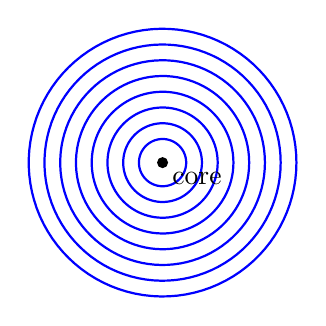
\begin{tikzpicture}
  % parameters
  \def\N{40} % number of streamlines
  \def\Rmax{2.0} % domain radius

  % Draw streamlines (circles around the origin)
  \foreach \r in {0.3,0.5,0.7,0.9,1.1,1.3,1.5,1.7} {
    \draw[blue, thick, domain=0:360, samples=100, variable=\t]
      plot ({\r*cos(\t)}, {\r*sin(\t)});
  }

  % Core marker
  \fill[black] (0,0) circle (2pt);
  \node[below right] at (0,0) {core};
\end{tikzpicture}

%--- Define a macro to draw pulsed waves at phase phi
\newcommand{\pulsedswirl}[1]{
\begin{tikzpicture}
  \def\Rmax{2.0}
  % Draw outward cosine-modulated ripples
  \foreach \r in {0.3,0.5,...,1.9} {
    \pgfmathsetmacro{\amp}{cos(10*\r - #1)} % wave oscillation
    \draw[thick, blue!70!black, opacity=0.8]
      (0,0) circle ({\r + 0.05*\amp});
  }
  % Core marker
  \fill[black] (0,0) circle (2pt);
\end{tikzpicture}
}

%--- Three snapshots ---
\pulsedswirl{0} % t = 0
\quad
\pulsedswirl{1.57} % t = π/2
\quad
\pulsedswirl{3.14} % t = π
